\begin{chapter}{Устойчивость двухкластерных вращательных режимов}
	\section{Устойчивость двухкластерных вращательных движений с постоянной расстройкой фаз}
	
	Перепишем \ref{pre-pend} в виде системы:
	
	\begin{equation} \label{system}
		\begin{cases}
			\dot{x} = y, \\
			\dot{y} = \frac{1}{m} \left[ (1 - 2\beta)\sin{\alpha}(1 - \cos{x}) - \sin{x}\cos{\alpha} - y \right]
		\end{cases}
	\end{equation}
	
	Выполним линеаризацию системы \ref{system}:
	
	\begin{equation} \label{system-linear}
		\begin{pmatrix}
			\dot{\hat{x}} \\
			\dot{\hat{y}}
		\end{pmatrix}
		=
		\begin{pmatrix}
			0 & 1 \\
			\frac{1}{m}\left[ (1 - 2\beta)\sin{\alpha}\sin{x_p} - \cos{\alpha}\cos{x_p} \right] & -\frac{1}{m}
		\end{pmatrix}
		\begin{pmatrix}
			\hat{x} \\
			\hat{y}
		\end{pmatrix}
	\end{equation}
	Где $x_p$ - стационарные состояния системы \ref{pre-pend}. Характеристический многочлен системы \ref{system-linear}:
	
	\begin{equation} \label{hp}
		\lambda^2 + \frac{1}{m}\lambda - \frac{1}{m}\left[ (1 - 2\beta)\sin{\alpha}\sin{x_p} - \cos{\alpha}\cos{x_p} \right] = 0
	\end{equation}
	
	Из \ref{hp} можно заметить, что устойчивость стационарного состояния $x_p$ определяется соотношением:
	
	\begin{equation} \label{hp-stability}
		\cos{\alpha}\cos{x_p} - (1 - 2\beta)\sin{\alpha}\sin{x_p} > 0
	\end{equation}
	
	Несложно заметить, что стационарные состояния в уравнении \ref{pre-pend} определяются выражением:
	$$
	\sin{(x_p + \varphi)} = \frac{(1 - 2\beta) \sin{\alpha}}{\sqrt{\cos{\alpha}^2 + (1 - 2\beta)^2\sin{\alpha}^2}},
	$$
	Откуда:
	\begin{equation} \label{x1}
		x_{p_1} = \begin{cases}
			0, \alpha \in [-\pi/2, \pi/2) \\
			2\arcsin{\frac{(1 - 2\beta) \sin{\alpha}}{\sqrt{\cos{\alpha}^2 + (1 - 2\beta)^2\sin{\alpha}^2}}} - \pi , \alpha \in [\pi/2, 3\pi/2)
		\end{cases}
	\end{equation}
	
	\begin{equation} \label{x2}
	x_{p_2} = \begin{cases}
		\pi - 2\arcsin{\frac{(1 - 2\beta) \sin{\alpha}}{\sqrt{\cos{\alpha}^2 + (1 - 2\beta)^2\sin{\alpha}^2}}}, \alpha \in [-\pi/2, \pi/2) \\
		0, \alpha \in [\pi/2, 3\pi/2)
		\end{cases}
	\end{equation}
	
	Подставляя \ref{x1}, \ref{x2} в \ref{hp-stability}
	получаем, что $x_{p_1}$ - устойчива, $x_{p_2}$ - неустойчива.

	\begin{figure}[h!]\center		
		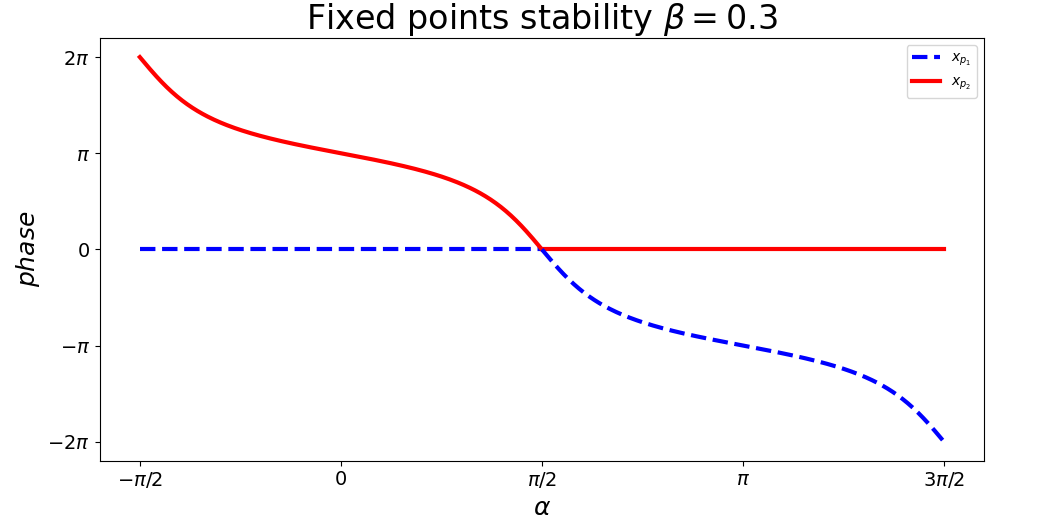
\includegraphics[width=1\columnwidth]{pictures/fixed-points.png} 
		\caption{\textbf{Устойчивость стационарных состояний.}
		Синяя пунктирная линия - устойчивое состояние $x_{p_1}$,
		Красная сплошная линия - неустойчивое состояние $x_{p_2}$.
		$\beta = 0.3$}
		\label{fp-2}
	\end{figure}

	\begin{figure}[h!]
		\begin{center}
			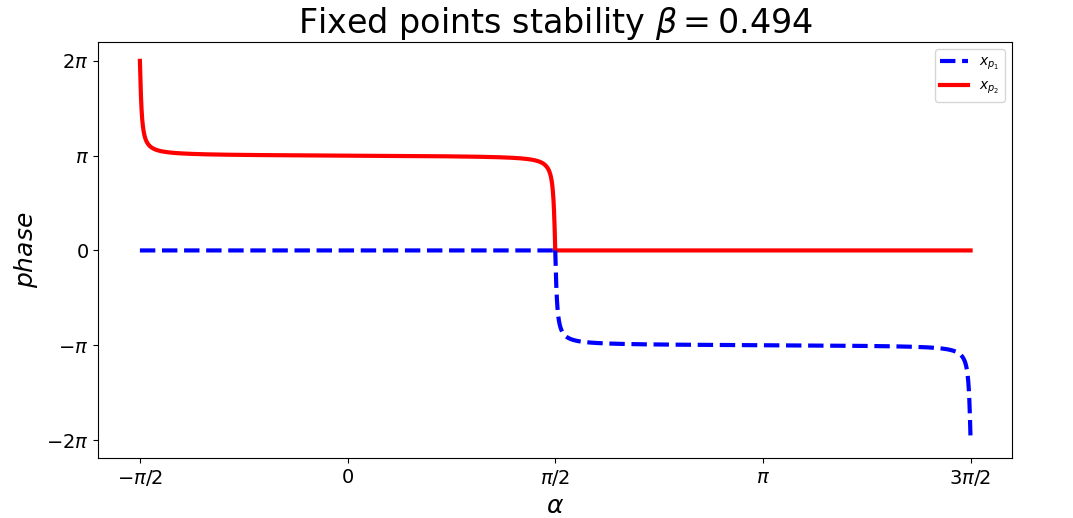
\includegraphics[width=1\columnwidth]{pictures/fixed-points-3.png}
		\end{center}
		\caption{\textbf{Устойчивость стационарных состояний.}
		Синяя пунктирная линия - устойчивое состояние $x_{p_1}$,
		Красная сплошная линия - неустойчивое состояние $x_{p_2}$.
		$\beta = 0.494$}
		\label{fp-3}
	\end{figure}

	На рисунке \ref{fp-2} изображены стационарные состояния уравнения \ref{pre-pend} при параметре $\beta = 0.3$.
	Синей пунктирной линией отмечены устойчивые стационарные состояния,
	красной сплошной - неустойчивые. При $\alpha \in [-\pi/2, \pi/2)$ $x_{p_1} = 0$ и является устойчивой, что соответствует
	устойчивому синфазному вращательному режиму в исходной системе. Это естественно, ведь при $\alpha \in [-\pi/2, \pi/2)$ связь является
	притягивающей. Заметим, что при $\beta$ стремящейся к 0.5 стационарные состояния с расстройкой фаз неравной нулю стремятся
	к $\pi k$, $k \in \mathbb{Z}$ (см.рис. \ref{fp-3}).
	Стоит отметить, что в полной системе \ref{main-sistem} двухкластерное вращательное движение с постоянной расстройкой фаз $X = x_{p_1}$
	может терять свою устойчивость. Данный эффект будет продемонстрирован в следующем разделе, посвященном устойчивости.
	Таким образом нас будет интересовать только устойчивость двухкластерных состояний с периодической расстройкой фаз.
	
	\section{Устойчивость двухкластерных вращательных движений с периодической расстройкой фаз}

	Выполним линеаризацию относительно произвольного вращательного движения $\psi_i$ с помощью замены $\varphi_i = \psi_i + \delta_i$, где вариации $\delta_i$ малы:
	\begin{equation} \label{pretubr}
		m\ddot{\delta}_i + \dot{\delta}_i = \frac{1}{N} \sum_{j = 1}^N \cos{(\psi_j - \psi_i - \alpha)} \cdot (\delta_j - \delta_i), \ i = \overline{1, N}
	\end{equation}
	Для случая двухкластерного режима \ref{two-cluster} система \ref{pretubr} запишется в виде:
	
	\begin{equation}
		\begin{cases}
			m\ddot{\delta}_i + \dot{\delta}_i = \frac{1}{N} \left( \cos{\alpha} \sum_{j = 1}^K (\delta_j - \delta_i) + \cos{(X + \alpha)} \sum_{j = K + 1}^N (\delta_j - \delta_i) \right), \ i = \overline{1,K}, \\
			m\ddot{\delta}_i + \dot{\delta}_i = \frac{1}{N} \left( \cos{(X - \alpha)} \sum_{j = 1}^K (\delta_j - \delta_i) +  \cos{\alpha} \sum_{j = K + 1}^N (\delta_j - \delta_i)  \right), \ i = \overline{K + 1,N},
		\end{cases}		
	\end{equation}
	
	Выполняя замену:
	\begin{align*}
		\eta_1 = \frac{1}{K} \sum_{i = 1}^K \delta_i - \frac{1}{N - K} \sum_{i = K + 1}^N \delta_i, \\
		\eta_2 = \frac{1}{K} \sum_{i = 1}^K \delta_i + \frac{1}{N - K} \sum_{i = K + 1}^N \delta_i, \\
		\xi_n = \delta_{n+1} - \delta_n, \ 1 \leq  n \leq K - 1, \\
		\zeta_n = \delta_{n+1} - \delta_n, \ K + 1 \leq n \leq N - 1.
	\end{align*}
		
	Приходим к системе уравнений:
	
	\begin{equation} \label{split-linear-pert-sys-n12}
		\begin{cases}
			m\ddot{\eta}_1 + \dot{\eta}_1 + \left( \beta \cos{(X - \alpha)} + (1 - \beta) \cos{(X + \alpha)} \right) \eta_1 = 0, \\
			m\ddot{\eta}_2 + \dot{\eta}_2 + \left( (1 - \beta) \cos{(X + \alpha)} - \beta \cos{(X - \alpha)} \right) \eta_1 = 0,
		\end{cases}
	\end{equation}
	
	
	\begin{equation} \label{split-linear-pert-sys-ksi-eta}
		\begin{cases}
			m\ddot{\xi}_n + \dot{\xi}_n + \left( (1 - \beta) \cos{(X + \alpha)} + \beta \cos{\alpha} \right) \xi_n = 0, \\
			m\ddot{\zeta}_n + \dot{\zeta}_n + \left( (1 - \beta) \cos{\alpha} + \beta \cos{(X - \alpha)} \right) \zeta_n = 0.
		\end{cases}
	\end{equation}
	
	Так как $X$ периодична, мы можем применить теорию Флоке
	и найти мультипликаторы, определяющие асимптотическое поведение решений системы.
	
	Проанализируем систему \ref{split-linear-pert-sys-n12} (переменные $\eta_1$, $\eta_2$).
	Из \ref{pre-pend} следует, что одним из
	решений первого уравнения является $\dot{X}$.
	Так как $X$ периодична, то один из мультипликаторов равен 1.
	Согласно формуле Лиувилля-Остроградского, второй мультипликатор первого уравнения равен $\exp{(-\frac{T_x}{m})}$.
	Кроме того, полная система имеет решение $\eta_1 = 0$, $\eta_2 = const$,
	откуда следует, что еще один мультипликатор равен единице.
	Вновь применяя формулу Лиувилля-Остроградского, но
	уже ко всей системе, находим четвертый мультипликатор,
	равный $\exp{(-\frac{T_x}{m})}$. 
	Итак, рассматриваемый режим всегда внутренне устойчив.

	
	Проанализируем систему \ref{split-linear-pert-sys-ksi-eta} (переменные $\xi$, $\zeta$).
	Переменная $\xi$ соответствует малому кластеру, переменная $\zeta$ соответствует большому кластеру. 
	Они не связанны между собой.
	Благодаря такому разделению переменных, мы можем проследить как меняется устойчивость
	двухкластерного режима с периодической расстройкой фаз для каждого кластера. В зависимости от $X$ устойчивость
	может пропасть или появится только у одного или сразу у двух кластеров, благодаря чему мы можем
	понять каким образом двухкластерный режим будет разрушаться в случае потери устойчивости.
	
	С помощью уравнений \ref{split-linear-pert-sys-ksi-eta} определим устойчивость стационарного
	двухкластерного вращательного режима, соответствующего состоянию $x_{p_1}$.
	Уравнения запишутся в виде:
	
	\begin{equation}
		x_{p_1} = 0, \ \alpha \in [-\pi/ 2, \pi/2]: 
		\begin{cases}
			m\ddot{\xi}_n + \dot{\xi}_n + \cos{\alpha}\xi_n = 0, \\
			m\ddot{\zeta}_n + \dot{\zeta}_n + \cos{\alpha}\zeta_n = 0.
		\end{cases}
	\end{equation}
	
	\begin{equation}
		\begin{split}
			x_{p_1} = 2\arcsin{\frac{(1 - 2\beta) \sin{\alpha}}{\sqrt{\cos{\alpha}^2 + (1 - 2\beta)^2\sin{\alpha}^2}}} - \pi , \alpha \in [\pi/2, 3\pi/2): \\ 
			:\begin{cases}
				m\ddot{\xi}_n + \dot{\xi}_n + A(\alpha, \beta) \xi_n = 0, \\
				m\ddot{\zeta}_n + \dot{\zeta}_n -A(\alpha, \beta) \zeta_n = 0.
			\end{cases}
		\end{split}
	\end{equation}
	Где $A$ - некоторый коэффициент. Заметим, что при $\alpha \in [-\pi/ 2, \pi/2)$, $x_{p_1}$ - устойчива в исходной системе,
	при $\alpha \in [\pi/2, 3\pi/2)$, $x_{p_1}$ - неустойчива в исходной системе.

	Получается, что в исходной системе двухкластерный вращательный режим с постоянной расстройкой фаз всегда является неустойчивым.
	Таким образом дальнейший анализ устойчивости мы будем проводить только для двухкластерных вращательных движений с периодической
	расстройкой фаз.


	В результате численного моделирования были получены карты устойчивости двухкластерных вращательных
	режимов с периодической расстройкой фаз в области параметров $\alpha$, $m$. Из рисунка \ref{map-083} видно, что устойчивость двухкластерного режима разрушается из - за потери устойчивости у одного из кластеров:
	как большого при больших значениях параметра $\alpha$, так и малого при меньших значениях параметра $\alpha$.
	Можно заметить, что внутри зоны устойчивости большого кластера появляется зона параметрической неустойчивости при $\beta \approx 0.25$, которая
	разрастается с увеличением параметра $\beta$. При $\beta \approx 0.375$ (см. рис. \ref{map-0375}) зона устойчивости большого кластера
	распадается на две несвязных компоненты. Данные результаты подтверждены прямым численным моделированием (см. рис. \ref{st-c-1}, \ref{st-c-2}, \ref{st-c-3}, \ref{st-c-4}).
	На рисунке \ref{su-map} изображена карта устойчивости двухкластерных вращательных состояний с
	периодической расстройкой фаз в зависимости от размеров малого кластера. Более темный цвет
	характеризуется большей мультистабильностью двухкластерных вращательных движений.
	Чем больше размер малого кластера, тем меньше соответствующая
	зона устойчивости. Также при увеличении размеров малого кластера увеличивается максимально возможное значение параметра
	$\alpha$, при котором двухкластерное вращательное движение сохраняет свою устойчивость.
	Наблюдается небольшая область устойчивости двухкластерного вращательного движения при параметрах $\alpha > \pi/2$, что соответствует
	реализации отталкивающей связи. При увеличении размеров малого кластера эта область также увеличивается в размерах.

	\begin{figure}[h!]\center
		
		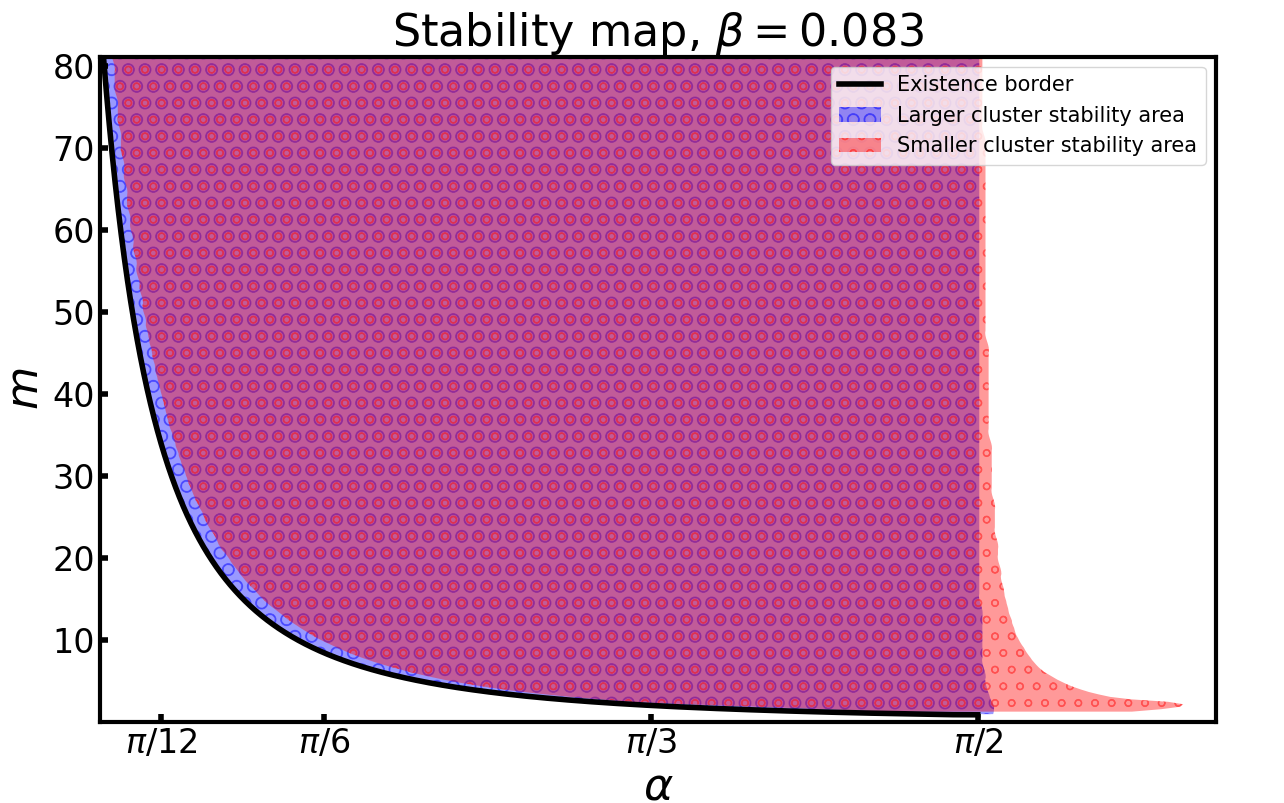
\includegraphics[width=1\columnwidth]{pictures/map-0-083.png}
		\caption{\textbf{Карта устойчивости двухкластерных вращательных состояний с периодической расстройкой фаз.}
		Область с малыми маркерами соответствует устойчивости малого кластера.
		Область с большими маркерами соответствует устойчивости большого кластера.
		На пересечении этих областей двухкластерный вращательный режим с периодической расстройкой фаз является устойчивым}
		\label{map-083}
	\end{figure}


	\begin{figure}[h!]\center
		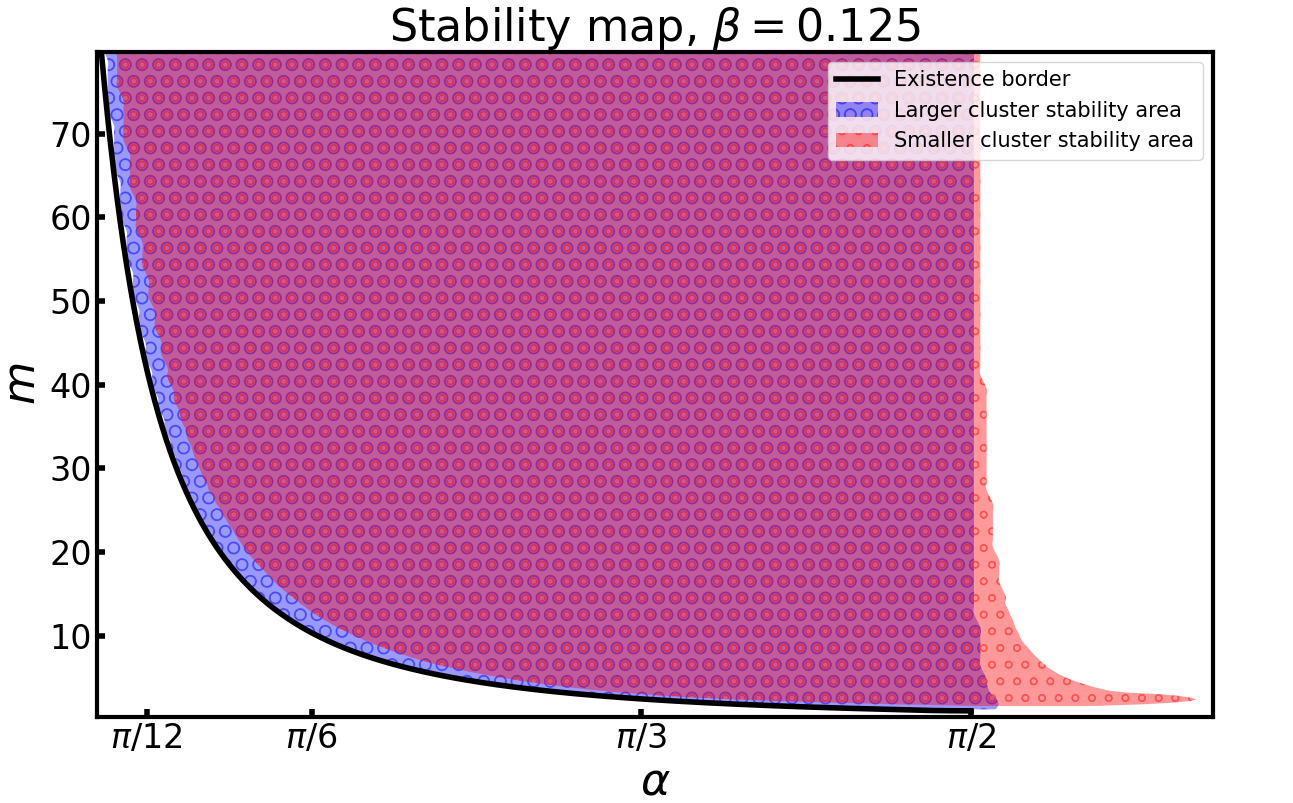
\includegraphics[width=1\columnwidth]{pictures/map-0-0125.png}
		\caption{\textbf{Карта устойчивости двухкластерных вращательных состояний с периодической расстройкой фаз.}
		Область с малыми маркерами соответствует устойчивости малого кластера.
		Область с большими маркерами соответствует устойчивости большого кластера.
		На пересечении этих областей двухкластерный вращательный режим с периодической расстройкой фаз является устойчивым}
		\label{map-0125}
	\end{figure}

	
	\begin{figure}[h!]\center
		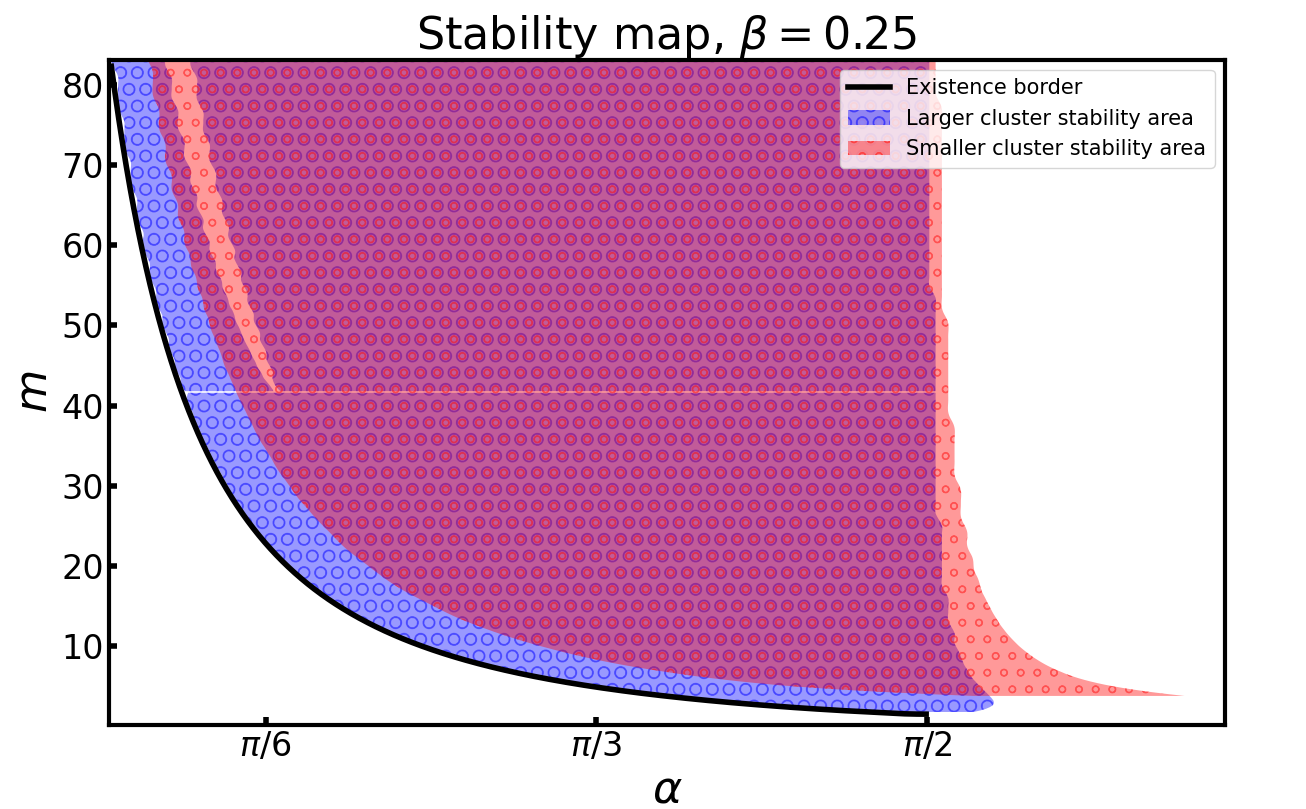
\includegraphics[width=1\columnwidth]{pictures/map-0-25.png}
		\caption{\textbf{Карта устойчивости двухкластерных вращательных состояний с периодической расстройкой фаз.}
		Область с малыми маркерами соответствует устойчивости малого кластера.
		Область с большими маркерами соответствует устойчивости большого кластера.
		На пересечении этих областей двухкластерный вращательный режим с периодической расстройкой фаз является устойчивым}
		\label{map-025}
	\end{figure}


	\begin{figure}[h!]\center
		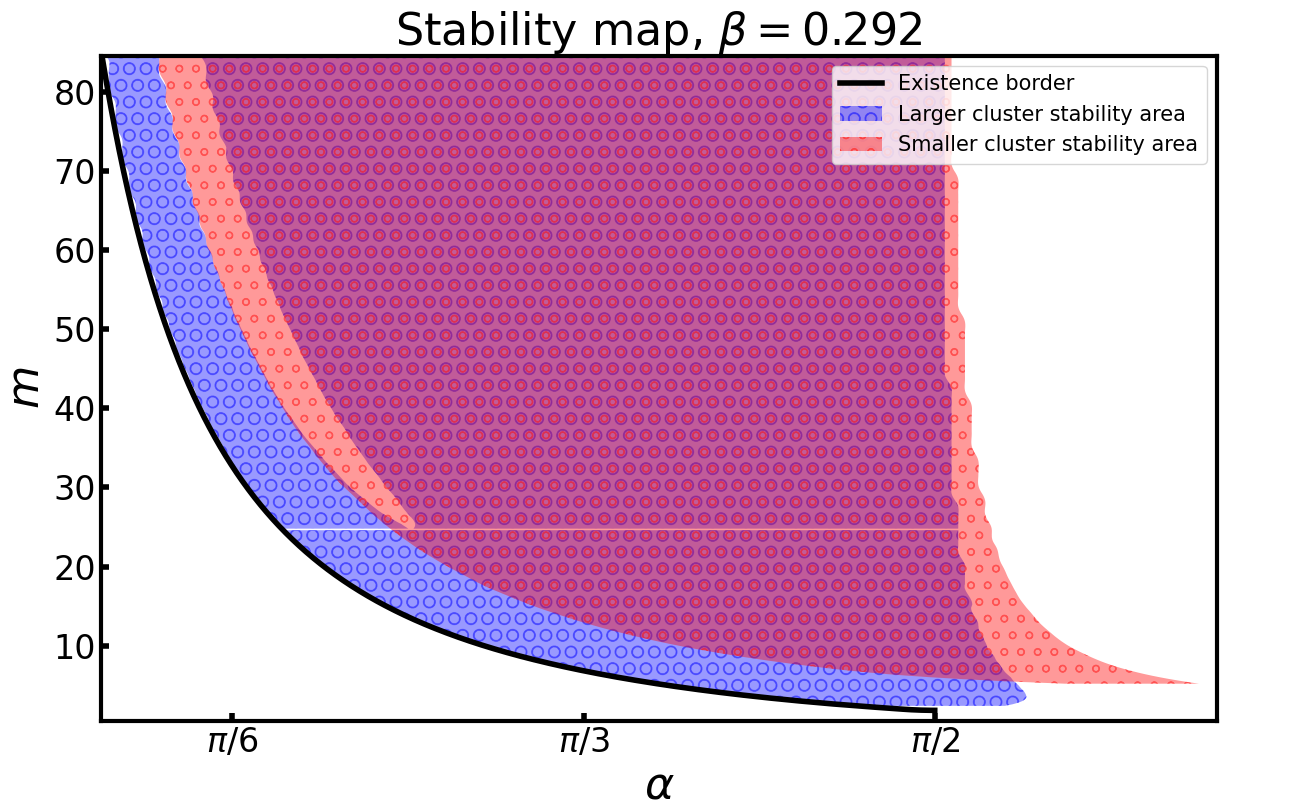
\includegraphics[width=1\columnwidth]{pictures/map-0-292.png}
		\caption{\textbf{Карта устойчивости двухкластерных вращательных состояний с периодической расстройкой фаз.}
		Область с малыми маркерами соответствует устойчивости малого кластера.
		Область с большими маркерами соответствует устойчивости большого кластера.
		На пересечении этих областей двухкластерный вращательный режим с периодической расстройкой фаз является устойчивым}
		\label{map-0-292}
	\end{figure}

	\begin{figure}[h!]\center
		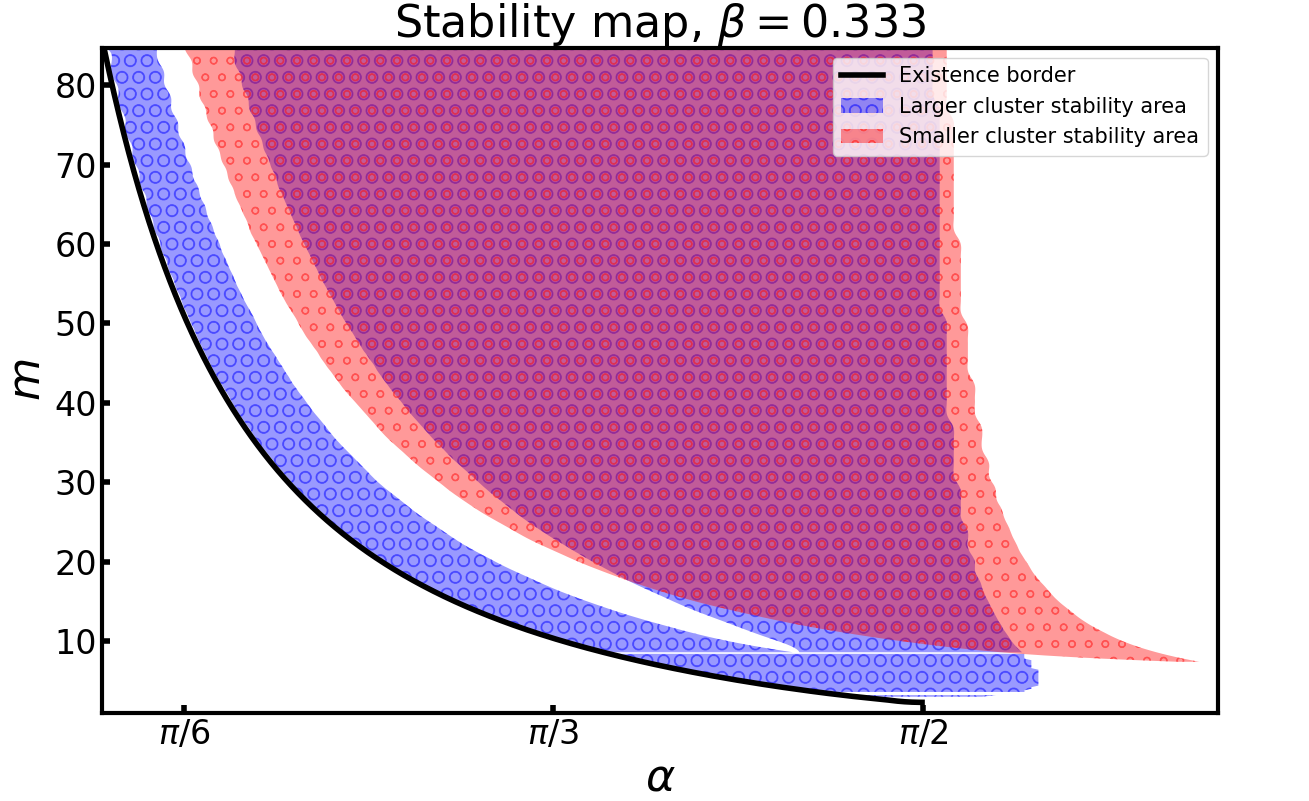
\includegraphics[width=1\columnwidth]{pictures/map-0-33.png}
		\caption{\textbf{Карта устойчивости двухкластерных вращательных состояний с периодической расстройкой фаз.}
		Область с малыми маркерами соответствует устойчивости малого кластера.
		Область с большими маркерами соответствует устойчивости большого кластера.
		На пересечении этих областей двухкластерный вращательный режим с периодической расстройкой фаз является устойчивым}
		\label{map-0-33}
	\end{figure}


	\begin{figure}[h!]\center
		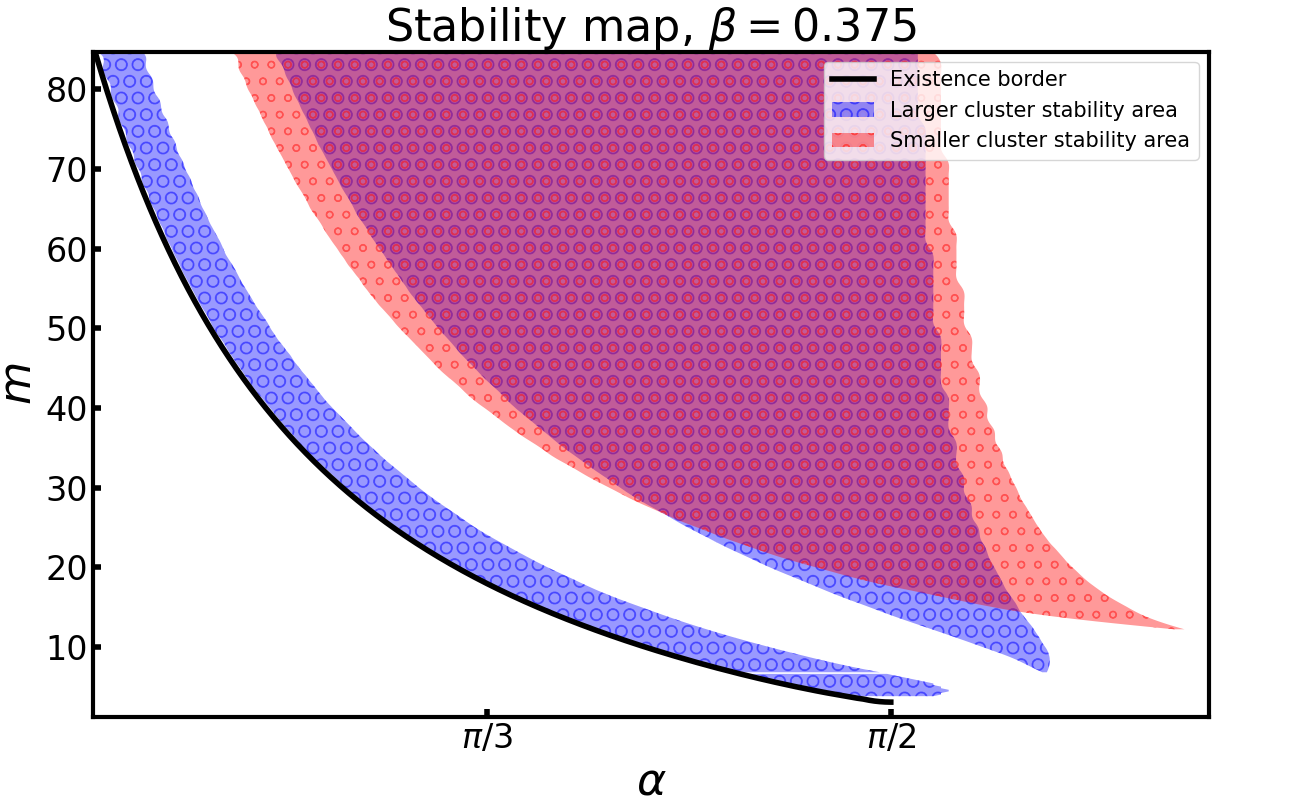
\includegraphics[width=1\columnwidth]{pictures/map-0-375.png}
		\caption{\textbf{Карта устойчивости двухкластерных вращательных состояний с периодической расстройкой фаз.}
		Область с малыми маркерами соответствует устойчивости малого кластера.
		Область с большими маркерами соответствует устойчивости большого кластера.
		На пересечении этих областей двухкластерный вращательный режим с периодической расстройкой фаз является устойчивым}
		\label{map-0375}
	\end{figure}

	\begin{figure}[h!]\center
		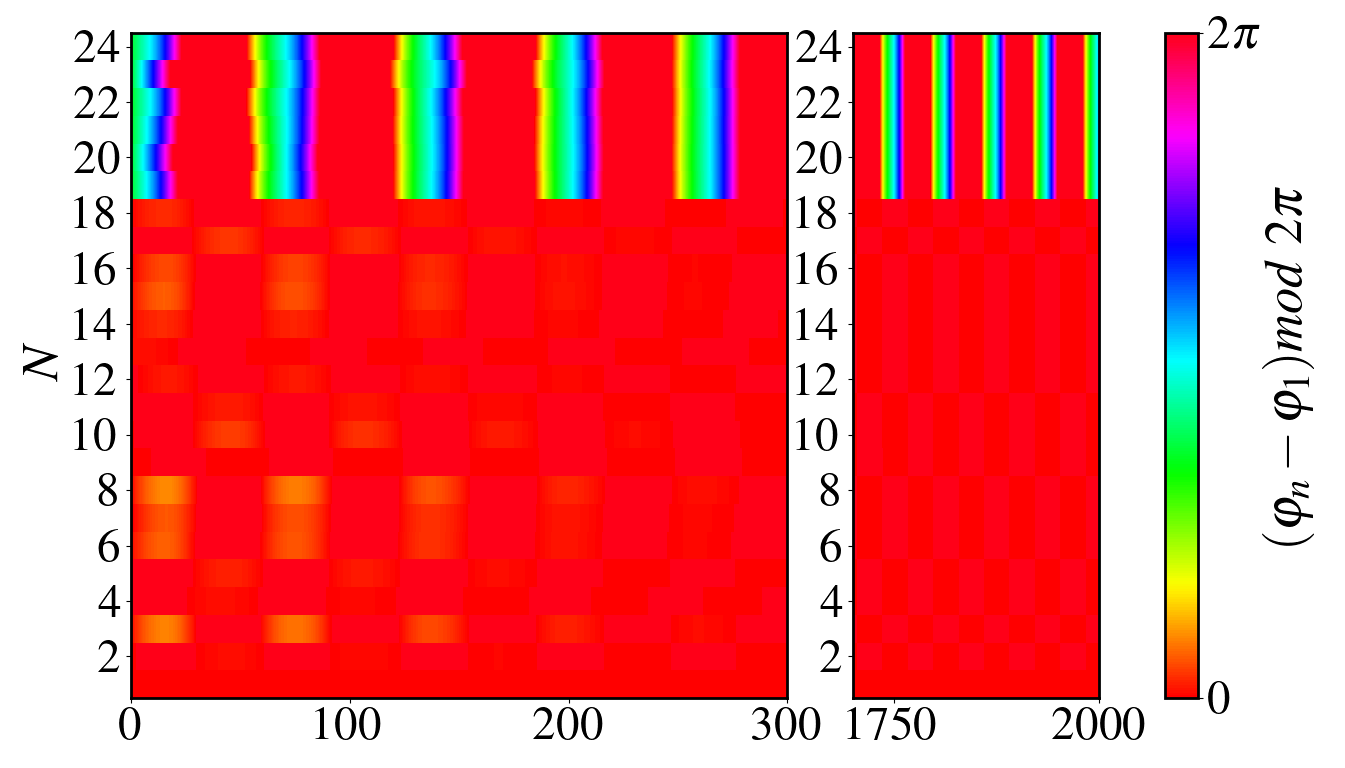
\includegraphics[width=1\columnwidth]{pictures/Figure_M_50_A_0.4586_O_1.png}
		\caption{\textbf{Пространственно-временная диаграмма.}
		Пространственно-временные диаграммы изображены для каждого элемента, относительно первого элемента.
		Цвет характеризует фазу элемента. Параметры: $N=24$, $m = 50$, $\omega = 1$, $\alpha = 0.4586$ (см. рис. \ref{map-025})}
		\label{st-c-1}
	\end{figure}

	\begin{figure}[h!]\center
		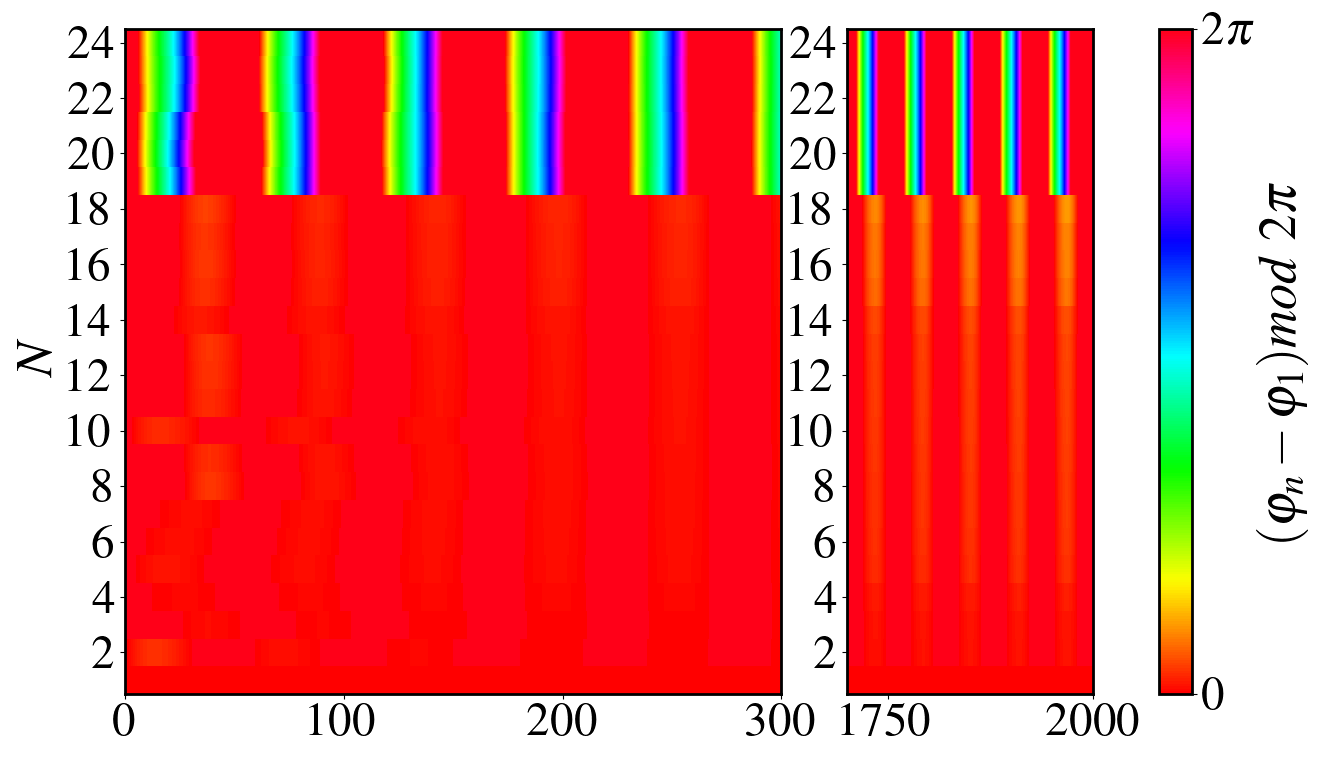
\includegraphics[width=1\columnwidth]{pictures/Figure_M_50_A_0.4946_O_1.png}
		\caption{\textbf{Пространственно-временная диаграмма.}
		Пространственно-временные диаграммы изображены для каждого элемента, относительно первого элемента.
		Цвет характеризует фазу элемента. Параметры: $N=24$, $m = 50$, $\omega = 1$, $\alpha = 0.4946$ (см. рис. \ref{map-025})}
		\label{st-c-2}
	\end{figure}

	\begin{figure}[h!]
		\begin{center}
			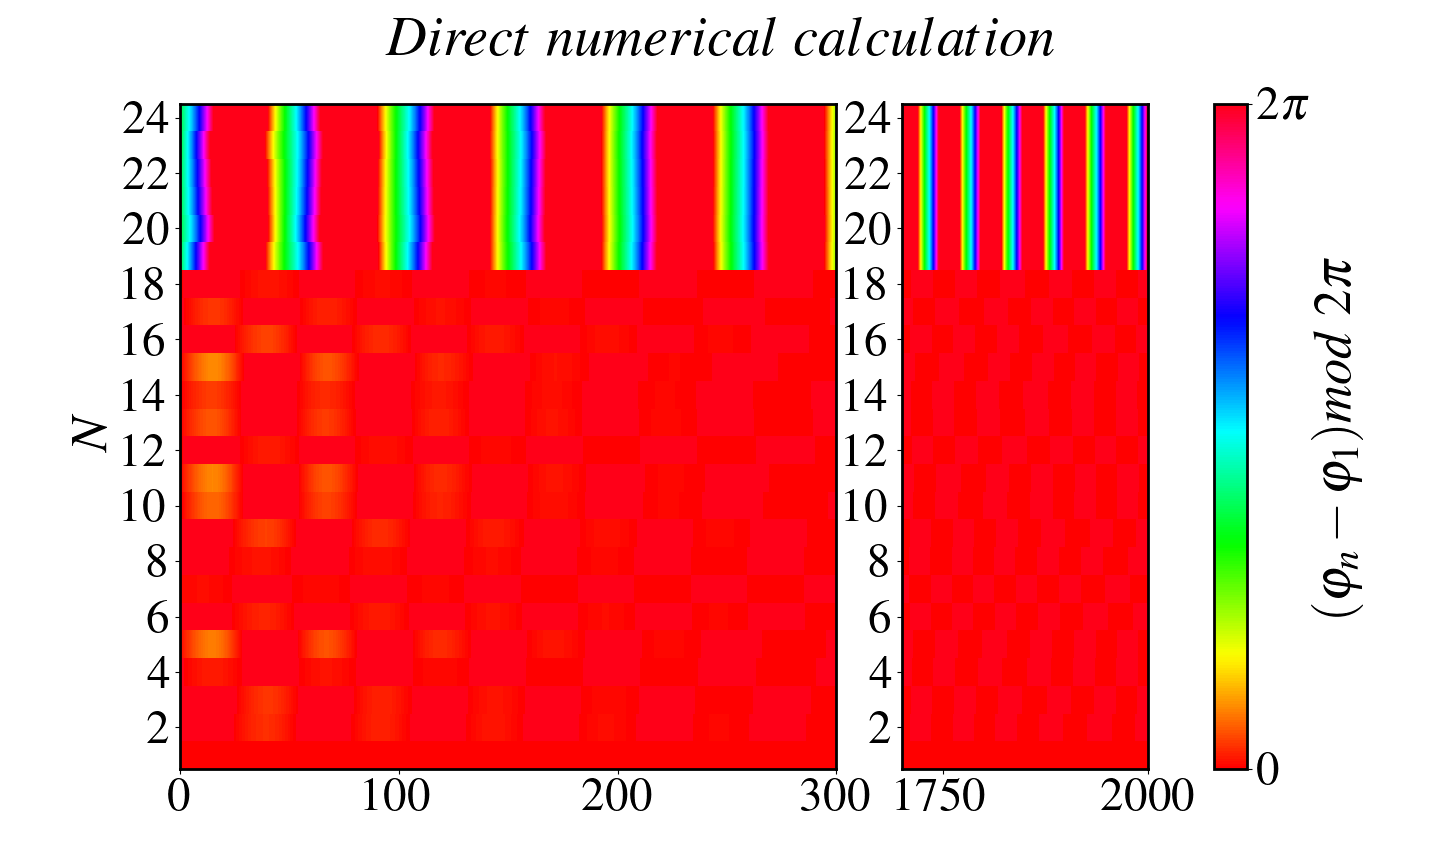
\includegraphics[width=1\columnwidth]{pictures/Figure_M_50_A_0.54_O_1.png}
		\end{center}
		\caption{\textbf{Пространственно-временная диаграмма.}
		Пространственно-временные диаграммы изображены для каждого элемента, относительно первого элемента.
		Цвет характеризует фазу элемента. Параметры: $N=24$, $m = 50$, $\omega = 1$, $\alpha = 0.54$ (см. рис. \ref{map-025})}
		\label{st-c-3}
	\end{figure}

	\begin{figure}[h!]
		\begin{center}
			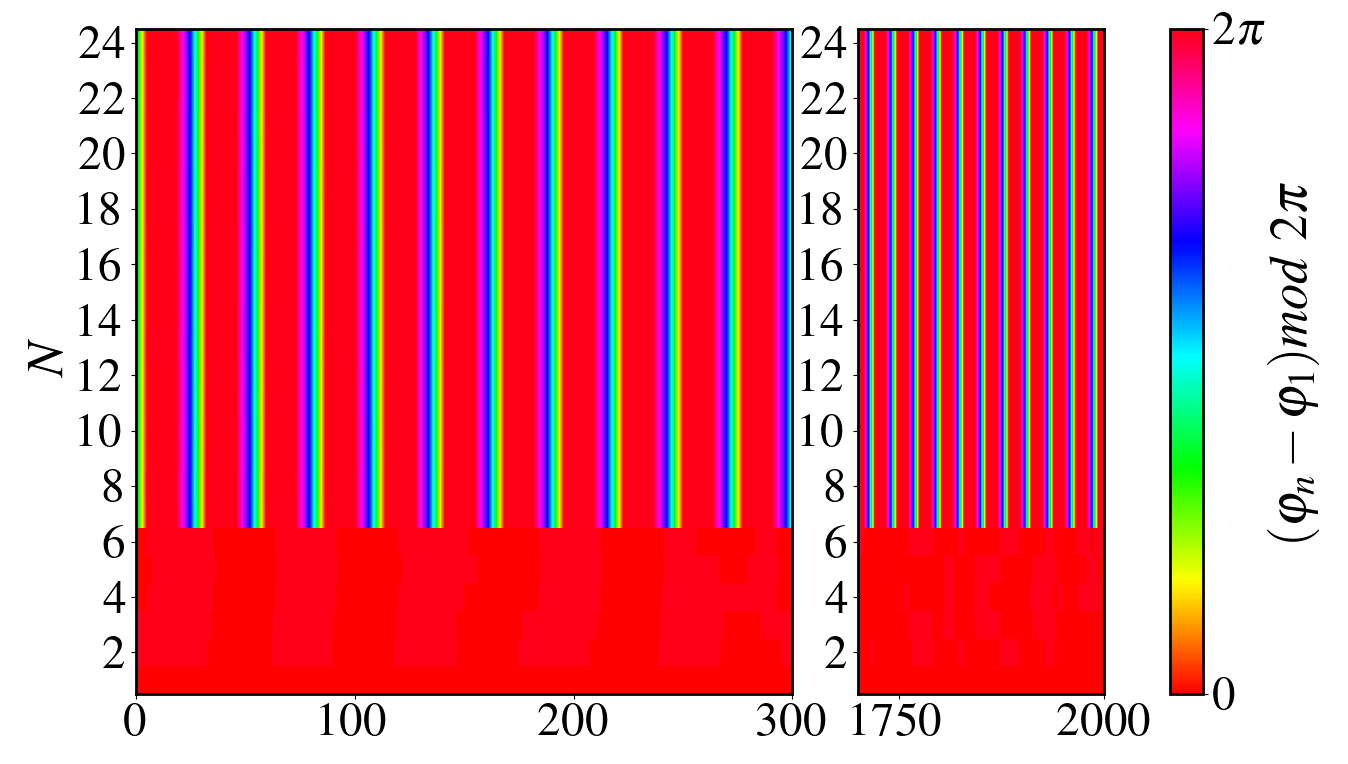
\includegraphics[width=1\columnwidth]{pictures/Figure_d.png}
		\end{center}
		\caption{\textbf{Пространственно-временная диаграмма.}
		Пространственно-временные диаграммы изображены для каждого элемента, относительно первого элемента.
		Цвет характеризует фазу элемента. Параметры: $N=24$, $m = 6.6$, $\omega = 1$, $\alpha = 1.6$ (см. рис. \ref{map-025})}
		\label{st-c-4}
	\end{figure}

	\begin{figure}[h!]
		\begin{center}
			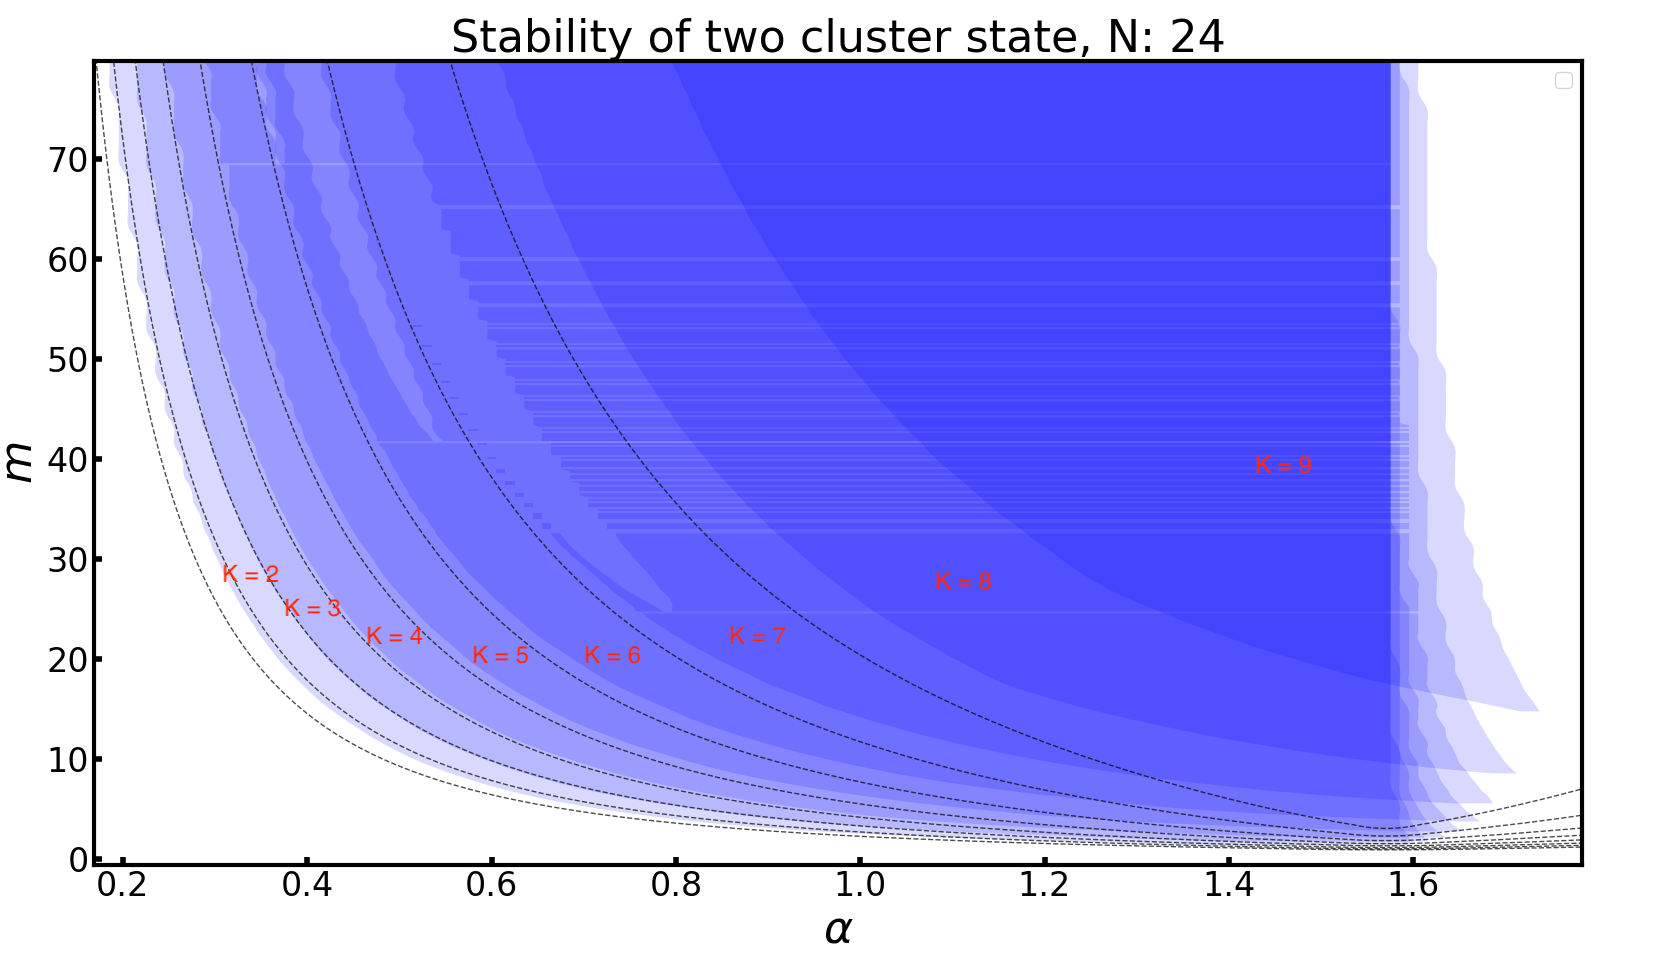
\includegraphics[width=1\columnwidth]{pictures/st-map.png}
		\end{center}
		\caption{\textbf{Карта устойчивости двухкластерных вращательных состояний с периодической расстройкой фаз в зависимости от размеров малого кластера.}
		Количество элементов $N = 24$. Внутри синей зоны двухкластерный режим является устойчивым. Черная пунктирная линия показывает
		границы существования двухкластерного вращательного режима. Текст, выделенный красным цветом, показывает количество элементов в малом
		кластере и располагается над соответствующей зоной устойчивости.}
		\label{su-map}
	\end{figure}

\end{chapter}